\documentclass[12pt,a4paper,fleqn]{article}
\title{Progress Report}
\author{Syed Ahmad Raza}
\date{2018.05.16}
\usepackage{mathtools}      % for math
\usepackage{graphicx}       % for graphics
%\usepackage{xcolor}         % for using colors in document
%\usepackage{afterpage}
\usepackage{float}          % force a figure placement with [H] command
%\usepackage{enumitem}       % control layout of itemize and enumerate
\usepackage{newtxtext}      % better text font
\usepackage{newtxmath}      % better math font
\usepackage{nicefrac}       % use nicer smaller fractions
%\usepackage{layouts}       % find \printinunitsof{in}\prntlen{\textwidth}
\graphicspath{{../figures/}}% only works when -shell-escape option is used

\begin{document}
\maketitle
%\tableofcontents
%\pagebreak

\section{Finite Volume Navier-Stokes solver}

\subsection{Final results for equal grid intervals}
A finite volume Navier-Stokes solver was coded in C++. The final results for various grid sizes are shown in the figures below.

\begin{figure}[H]
    \centering
    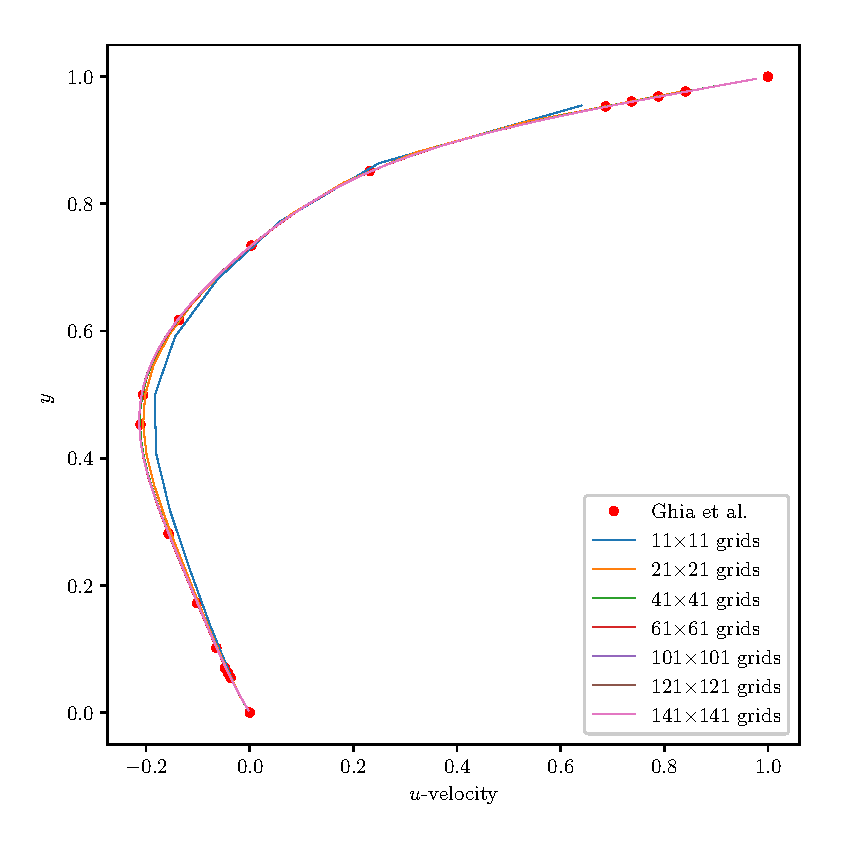
\includegraphics[width=\linewidth]{final18051412_cavityFlowU.eps}
    \caption{\(x\)-direction velocities at the center of \(x\)-axis are plotted against \(y\)-coordinates for various grid sizes, and compared with the results of Ghia et al.}
\end{figure}

\begin{figure}[H]
    \centering
    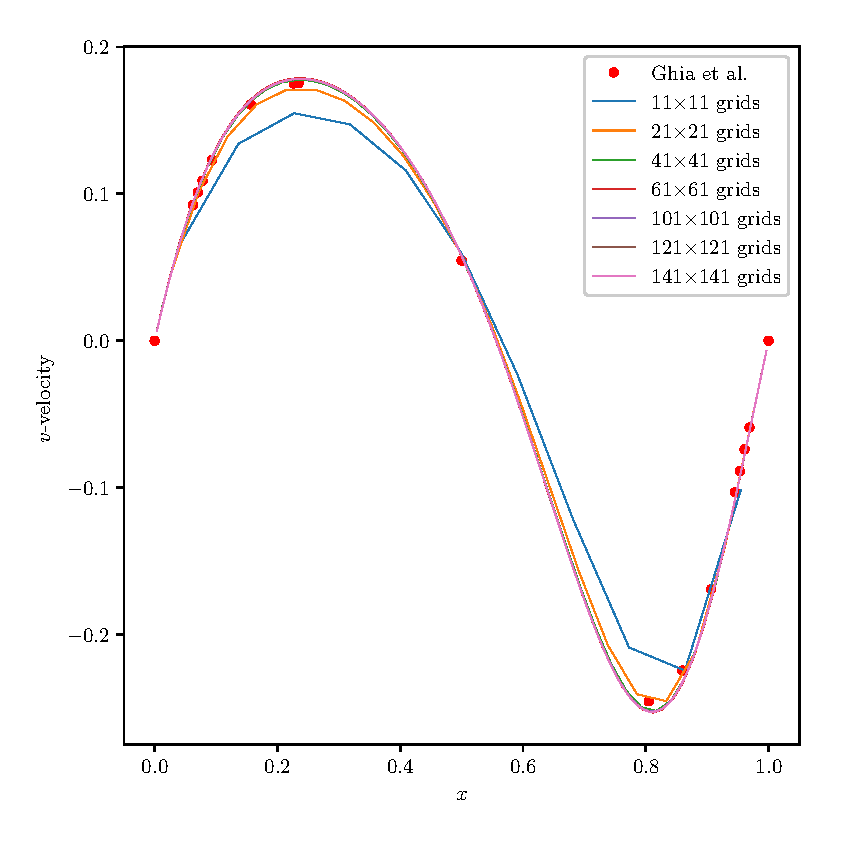
\includegraphics[width=\linewidth]{final18051412_cavityFlowV.eps}
        \caption{\(y\)-direction velocities at the center of \(y\)-axis are plotted against \(x\)-coordinates for various grid sizes, and compared with the results of Ghia et al.}
\end{figure}

The code has been modified to produce data files in a format that can be used in ParaView for plotting requirements. The velocity vector plot produced using ParaView is shown below.

\begin{figure}[H]
    \centering
    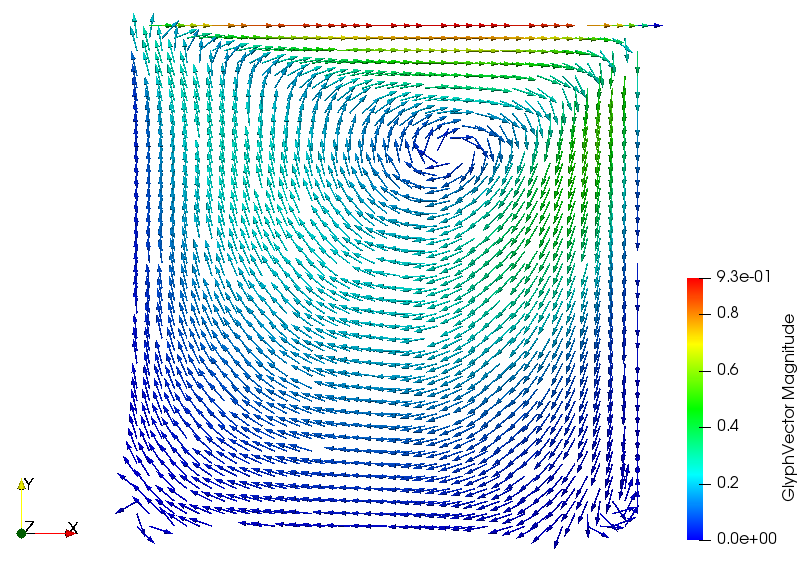
\includegraphics[width=\linewidth]{velVectors.png}
    \caption{Velocity vectors plotted using ParaView}
\end{figure}

\pagebreak

\subsection{Results for unequal grid intervals}
A grid with unequal grid intervals was used to test the code. The results are shown in the figures below.

\begin{figure}[H]
    \centering
    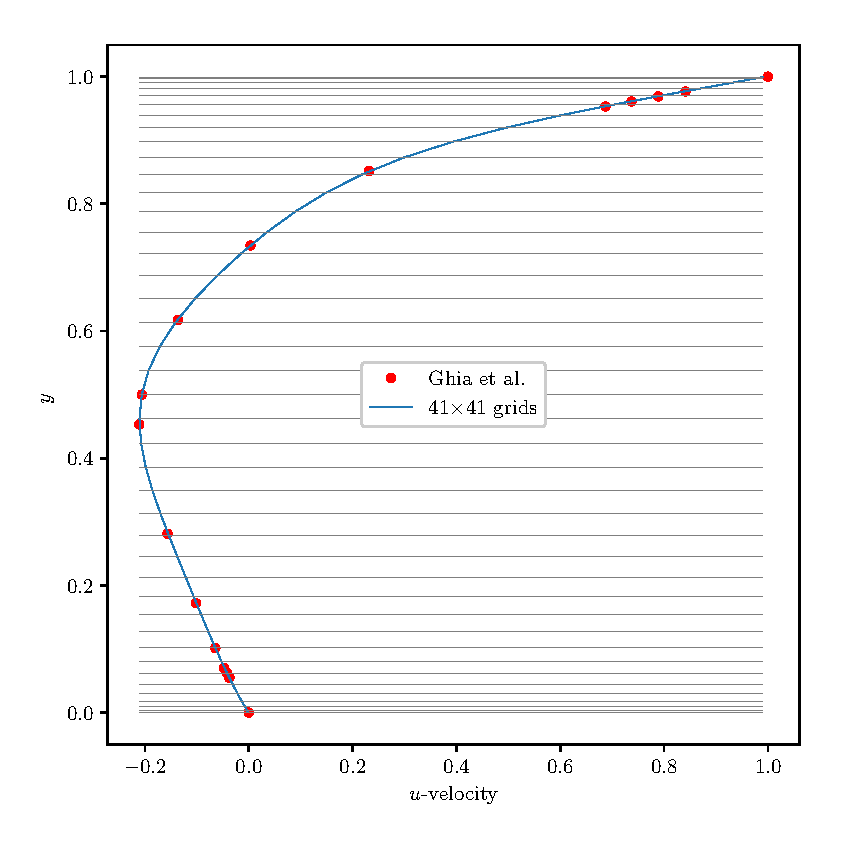
\includegraphics[width=\linewidth]{unequal_cavityFlowU.eps}
    \caption{\(x\)-direction velocities at the center of \(x\)-axis are plotted against \(y\)-coordinates for unequal grid sizes, and compared with the results of Ghia et al.}
\end{figure}

\begin{figure}[H]
    \centering
    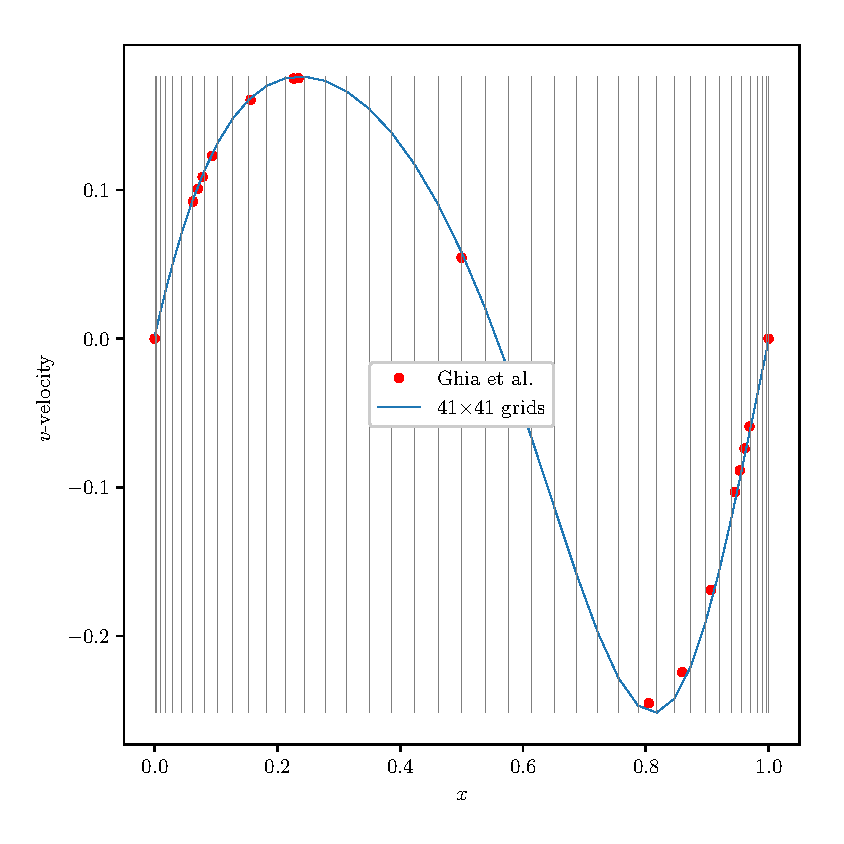
\includegraphics[width=\linewidth]{unequal_cavityFlowV.eps}
    \caption{\(y\)-direction velocities at the center of \(y\)-axis are plotted against \(x\)-coordinates for unequal grid sizes, and compared with the results of Ghia et al.}
\end{figure}

\subsection{Ongoing tasks}
\begin{enumerate}
    \item Calculating the virtual force for a cylinder inside a lid-driven cavity
    \item Converting the code for use with parallel computing using OpenMP
    \item Solve cavity-driven flow for 3D
\end{enumerate}

\end{document}
